
% this file is called up by thesis.tex
% content in this file will be fed into the main document

%: ----------------------- introduction file header -----------------------
\chapter{Introduction}

% ----------------------------------------------------------------------
%: ----------------------- introduction content ----------------------- 
% ----------------------------------------------------------------------



%: ----------------------- HELP: latex document organisation
% the commands below help you to subdivide and organise your thesis
%    \chapter{}       = level 1, top level
%    \section{}       = level 2
%    \subsection{}    = level 3
%    \subsubsection{} = level 4
% note that everything after the percentage sign is hidden from output

% TODO this is more of a background, the introduction should be an
% overview of the report.

The KM3NeT or the Cubic Kilometer Neutrino Telescope is currently being
constructed at the bottom of the Mediterranean Sea. The goal of this telescope
is two fold: first is to study high energy neutrinos originating from celestial
events such as birth of a neutrino star or a supernova. And second, to study
the properties of the neutrino particles produced in the Earth's atmosphere
\cite{adrian2016letter}. The first goal will be realized with the KM3NeT/ARCA
(Astroparticle Research with Cosmics in the Abyss) telescope and the second
with KM3NeT/ORCA (Oscillation Research with Cosmics in the Abyss)
\cite{adrian2016letter}. In this paper, we talk exclusively about KM3NeT/ARCA.

\begin{figure}[h]
  \centering
  \includegraphics[width=\textwidth]{blocks.jpg}
  \caption{Artist's impression of the ARCA detector \textit{source: https://www.km3net.org}}%
  \label{fig:blocks}
\end{figure}

The ARCA telescope comprises of two ``blocks'' with a total volume of
$1km^{3}$. Each block consists of 115 spherical detector units (DOMs)
and each DOM consists of 31 Photo Multiplier Tubes (PMTs) in various
spacial arrangement. Figure \ref{fig:blocks} shows an artist's
impression of ARCA, figure \ref{fig:doms} depicts a DOM along with the
PMTs inside it.

\begin{wrapfigure}{l}{0.5\textwidth}
  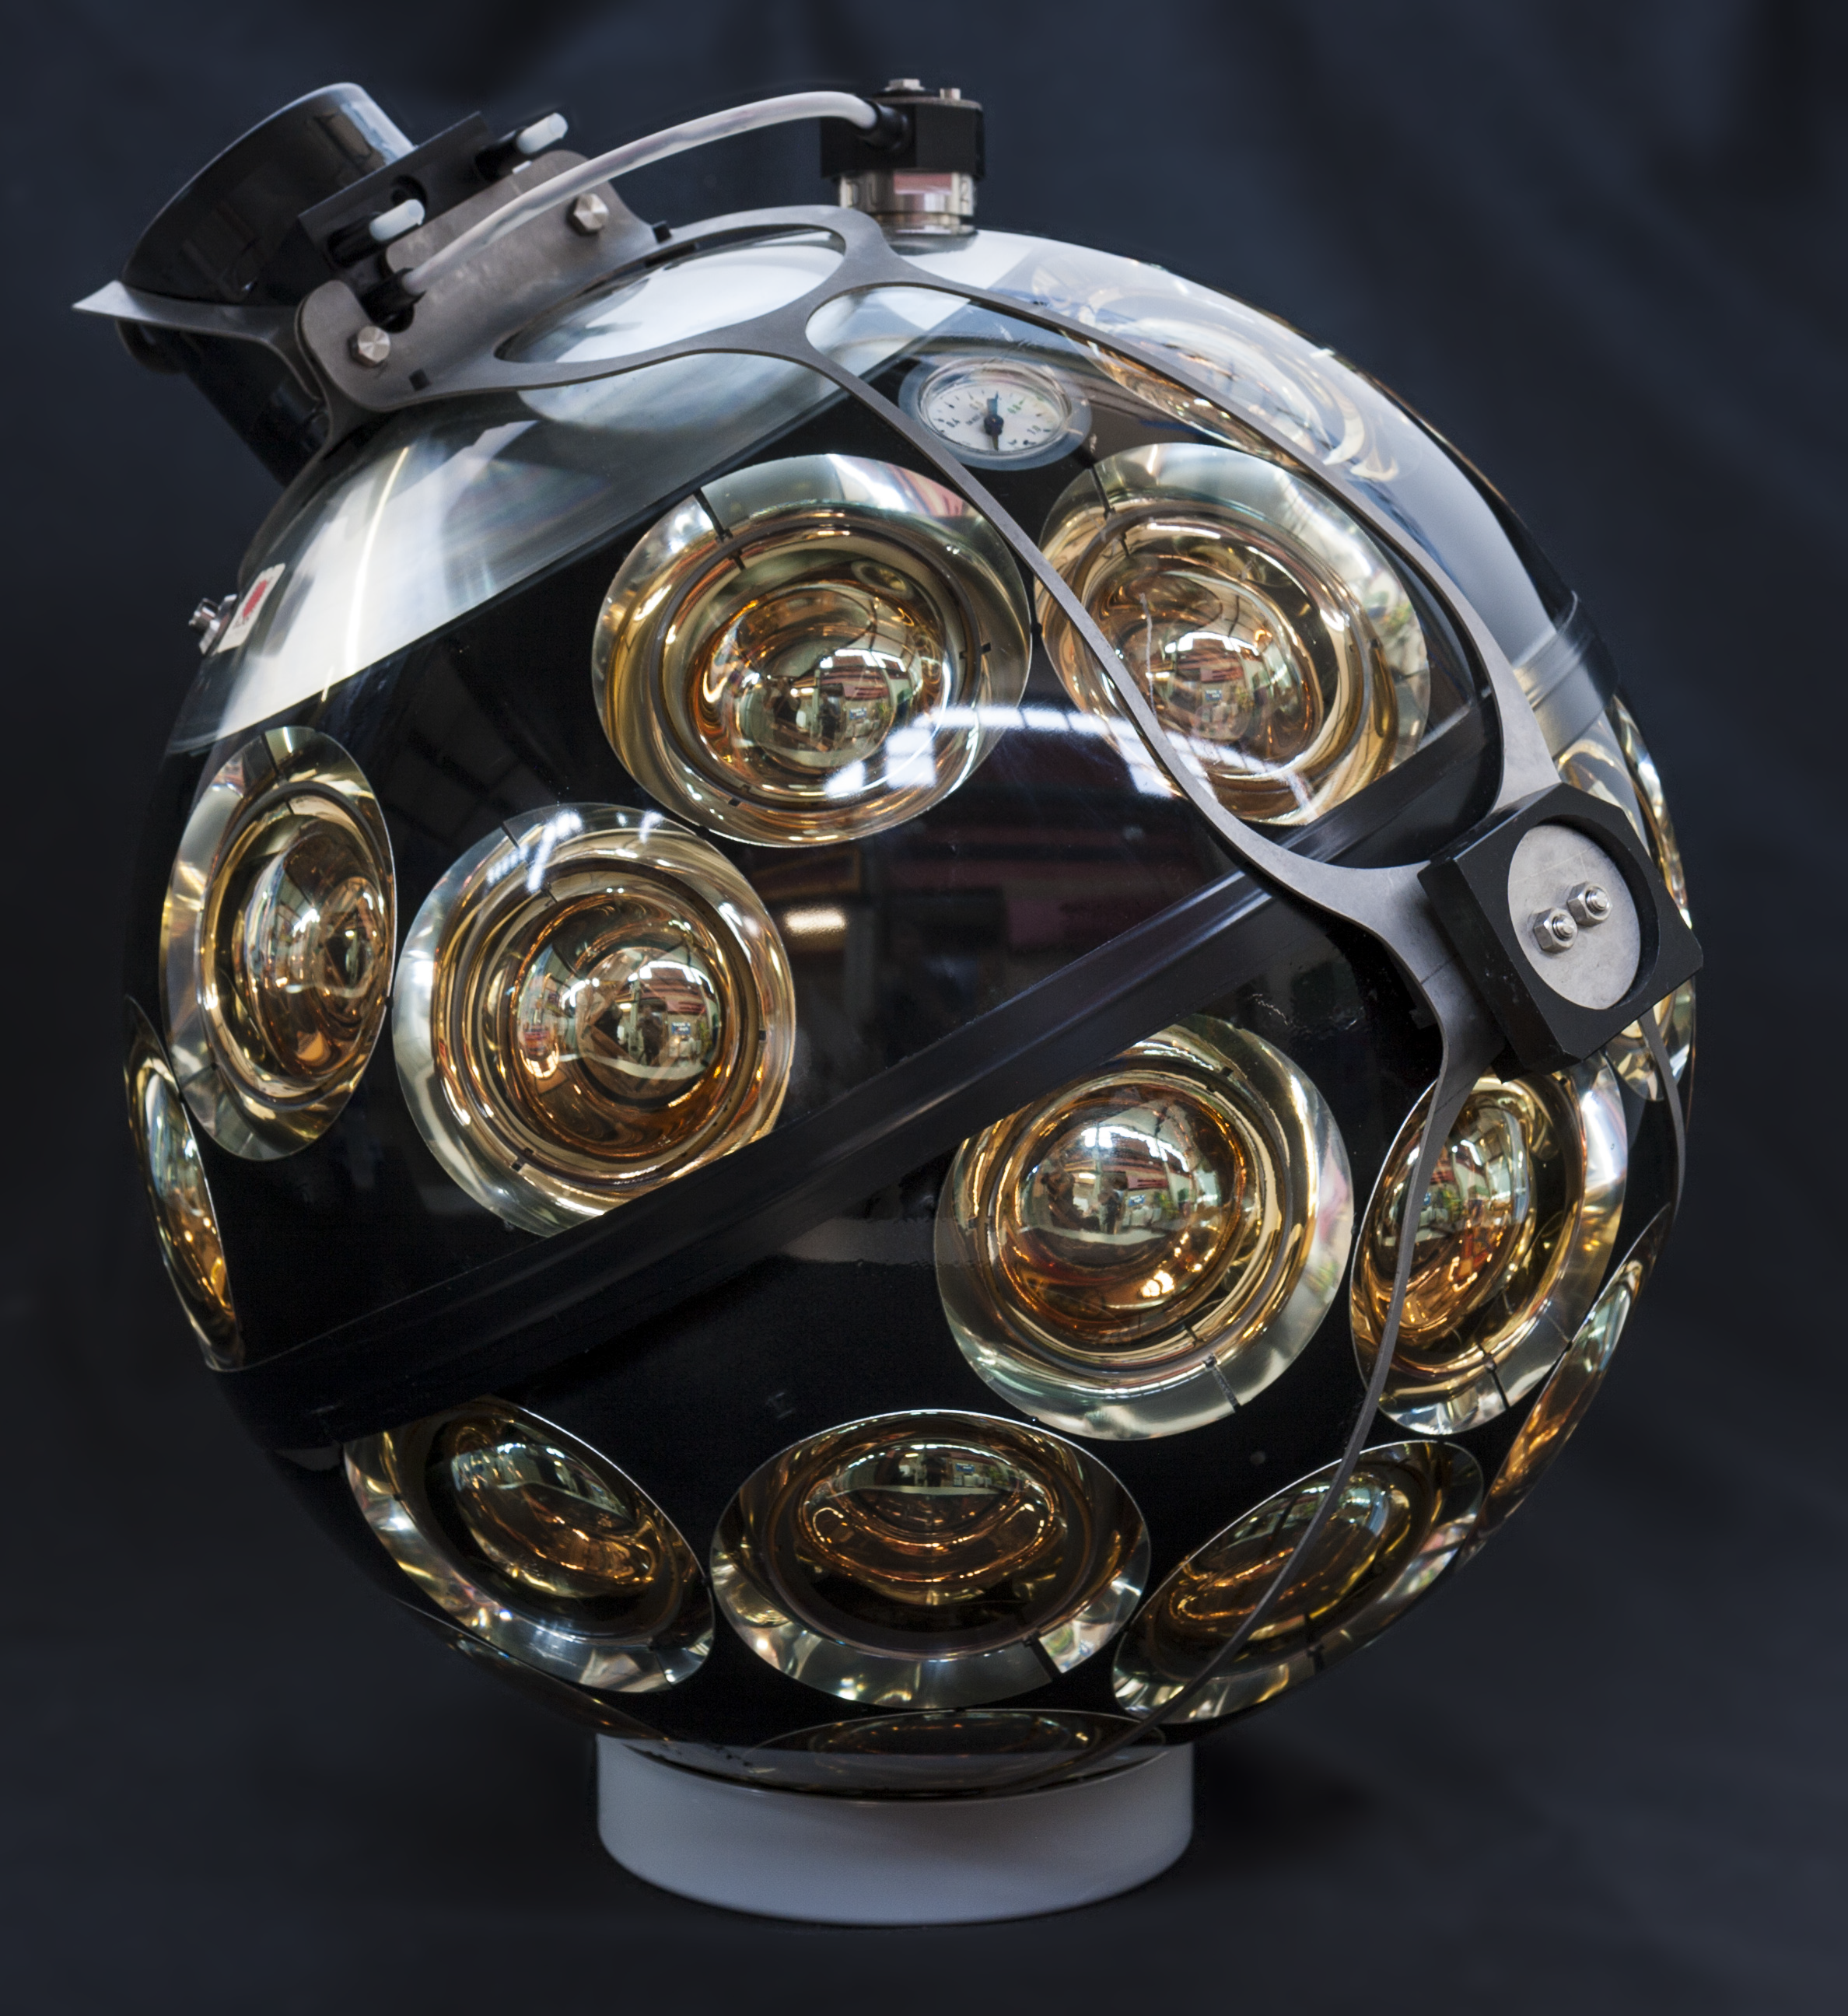
\includegraphics[width=0.9\linewidth]{doms.png}
  \caption{An optical detector (DOM) \textit{source: https://www.km3net.org}}%
  \label{fig:doms}
\end{wrapfigure}

The PMTs are sensitive to light or photons, the analog signal for all hits
above a certain threshold are digitized. This datapoint consists of a timestamp
and the spatial orientation of the DOM (ie. x,y,z coordinates). The digital
signals from all PMTs are arranged in 100ms ``timeslices'' and sent to the
on-shore facility for further processing \cite{aiello2019km3net}.

\section{Situation of Concern}

When the high energy neutrino particles interact with surrounding matter,
produce an electron and a photon, this phenomenon is known as the Cherenkov
Radiation or Cherenkov Light \cite{margiotta2014km3net}. This phenomenon is
utilized in the KM3NeT telescopes to detect high energy neutrinos ie. the
Cherenkov Light is detected by the PMTs. Unfortunately, there are several
sources of noise (in this case, the noise is other light sources),
bioluminescense and decay of Potassium 40 ($^{40}K$) and atmospheric Muons being
the primary sources \cite{post2019km3nnet}.

\subsection{State of the Art}\label{state-of-the-art}

Due to the high level of noise, data is generated at an extremely high rate of
25GB/sec \cite{adrian2016letter}. Due to this high data rate, it must be
filtered and selectively stored for further analysis. The state of the art for
this task are known as ``Event Trigger'' algorithms
\cite{adrian2016letter,aiello2019km3net}. The existing event trigger algorithms
namely \emph{L1} and \emph{L2} have limitations and can be improved upon
\cite{karas2019data}.

There is a tradeoff between performance and quality of the event trigger
algorithms to be realized here. The state of the art \emph{L1} and \emph{L2}
algorithms are very performant with the ability to filter data in real time
however their quality of filtration can be improved. Thus new event trigger
algorithms must consider this trade off.

Efforts have already been made to improve the existing event trigger
algorithms. \cite{karas2019data} proposed and implemented a GPU powered
pipeline which utilizes correlation and graph community detection to identify
time slices that may contain neutrino hits whilst \cite{post2019km3nnet}
suggests an alternate using convolutional neural networks.

% TODO here is an alternative to introduce related work chapter
Next chapter discusses the existing body of work on the matter.
Emphasis is put on the work done by \citeauthor{karas2019data} since
this project seeks to directly improve upon their work.

\subsection{User Requirements}\label{user-requirements}

The primary users of the ARCA are researchers who want to study high energy
particles from outer space. The stakeholders are all member institutes involved
in the project and by extension all scientists from these institutes who will
be working with the data collected.

The requirements of the primary users (and stakeholders) with respect to the
data acquisition pipeline are as follows.

\begin{enumerate}
  \item[\textbf{UR1}.]\textbf{The accuracy of filtration must be extremely high.}

    Time slices which are deemed important by event trigger algorithms
    are stored for further analysis and research. Failure to store
    time slices containing information from neutrino events can lead
    to loss of important data and thus a poor quality of research. On
    the other hand, since majority of the data generated is noise, the
    pipeline must be able to eliminate majority of noise to prevent
    storage of unnecessary and potentially useless data.

  \item[\textbf{UR2}.] \textbf{Filtration should occur in real time.}

    The state of the art event trigger algorithms are able to process
    data in real time. The proposed alternative ideally should
    maintain or improve upon it's predecessor's performance else
    provide a good trade off with data quality.

\end{enumerate}

\section{Research Question}
% TODO this section needs more work, iterate as and when possible
This report intends to improve upon the GPU pipeline proposed by
\citeauthor{karas2019data}, an overview for which is presented in
Chapter \ref{cha:karas-pipeline}. Specifically this project wishes to
answer the following research questions.

\begin{enumerate}
  \item[\textbf{RQ1}.] \textbf{Can the existing GPU pipeline be improved using neural networks (NNs)?}

    Improvement may be achieved by reducing the processing time of the
    pipeline or improving the accuracy of identifying important
    timeslices. This project focuses on achieving improvement via
    accuracy. The task of validating the runtime performance of the
    methods proposed in this paper is left to a separate project.

    In order to answer \textbf{RQ1}, the following sub questions are
    formulated.

  \item[\textbf{RQ2.}] \textbf{Can the \emph{Pattern Matrix Criterion} be replaced with a Multi Layer Perceptron?}

    \citeauthor{karas2019data} proposed a novel trigger criterion
    which given a pair of points, can quantify the level of
    correlation amongst the points with an accuracy of 80\%. The first
    phase of this project focuses on achieving better accuracy to
    identify ``causally related'' points using a Multi Layer
    Perceptron (MLP).
    % TODO introduce causally related points before reference here
    
  \item[\textbf{RQ3.}] \textbf{Can the \emph{Graph Community Detection} step be replaced with a Graph Convolusional Neural Network?}

    The output of the Pattern Matrix Criterion is used to create a
    graph structure where hits (of events and noise) are represented
    as nodes and causally related nodes are connected with an
    undirected edge carrying the probability of correlation as its
    weight. The Constant Pots clustering algorithm \cite{CITEME},
    which operates on the principles of Graph Community Detection, is
    used to separate the graph into communities of event and noise
    hits. The second phase of this project focuses on achieving a
    better accuracy for identifying event hits in a given timeslice
    using Graph Convolusional Neural Networks (GCNs).
    
\end{enumerate}
